

%and the Laplacian of any scalar function $f$ is 
%\[
%\Delta f = \frac{1}{r} \frac{\partial }{\partial r} \left( r  \frac{\partial f}{\partial r} \right) 
%+  \frac{1}{r^2} \frac{\partial^2 f}{\partial \theta^2} 
%\]

We seek an exact solution to the incompressible Stokes equations for an isoviscous, isothermal fluid in an  annulus.Given the geometry of the problem, we work in polar coordinates.
We denote the orthonormal basis vectors by $\mathbf{ e}_r$ and $\mathbf{ e}_\theta$, the inner radius of the annulus by $R_1$ and the outer radius by $R_2$.
Further, we assume that the viscosity $\mu$ is constant, which we set to $\mu = 1$ we set the gravity vector to $\mathbf{g} = -g_r \, \mathbf{e}_r$ with $g_r = 1$. 

Given these assumptions, the incompressible Stokes equations in the annulus are~\cite{scto01}
\begin{eqnarray}
A_r =     \frac{\partial^2 v_r}{\partial r^2} + \frac{1}{r} \frac{\partial v_r}{\partial r} +   
      \frac{1}{r^2} \frac{\partial^2 v_r}{\partial \theta^2}
    - \frac{v_r}{r^2} - \frac{2}{r^2} \frac{\partial u_\theta}{\partial \theta} 
-\frac{\partial p}{\partial r}  &=& \rho g_r \label{eq1} \\
A_\theta=
\frac{\partial^2 v_\theta}{\partial r^2} + \frac{1}{r} \frac{\partial v_\theta}{\partial r} + \frac{1}{r^2} \frac{\partial^2 v_\theta}{\partial \theta^2}
+\frac{2}{r^2} \frac{\partial v_r}{\partial \theta} - \frac{v_\theta}{r^2} 
-\frac{1}{r}\frac{\partial p}{\partial \theta} &=& 0
\label{eq2} \\
\frac{1}{r} \frac{\partial (rv_r)}{\partial r} + \frac{1}{r} \frac{\partial v_\theta}{\partial \theta} &=&0 \label{eq3}
\end{eqnarray}
Equations (\ref{eq1}) and (\ref{eq2}) are the momentum equations in polar coordinates while
Equation (\ref{eq3}) is the incompressibility constraint. 
The components of the velocity are obtained from the stream function as follows:
\[
v_r = \frac{1}{r}\frac{\partial \Psi}{\partial \theta}
\quad\quad
v_\theta = - \frac{\partial \Psi}{\partial r}
\]
where $v_r$ is the radial component and $v_\theta$ is the tangential component of the velocity vector.

The stream function is defined for incompressible (divergence-free) 
flows in 2D (as well as in 3D with axisymmetry).
The stream function can be used to plot streamlines, 
which represent the trajectories of particles in a steady flow.
From calculus it is known that the gradient vector $\nabla \Psi$
is normal to the curve $\Psi =C$. 
It can be shown that everywhere ${\boldsymbol {u}}\cdot \nabla \Psi =0$ 
using the formula for $\boldsymbol{u}$ in terms of 
$\Psi$ which proves that level curves of $\Psi$ are streamlines:
\[
{\bm u}\cdot \nabla \Psi 
= v_r \frac{\partial \Psi}{\partial r} + v_\theta \frac{1}{r} \frac{\partial \Psi}{\partial \theta} 
= \frac{1}{r}\frac{\partial \Psi}{\partial \theta} \frac{\partial \Psi}{\partial r} 
- \frac{\partial \Psi}{\partial r} \frac{1}{r} \frac{\partial \Psi}{\partial \theta} 
=0
\] 





In polar coordinates the curl of a vector ${\bm A}$ is:
\[
{\bm \nabla}\times {\bm A}
=
\frac{1}{r}\left(  
\frac{\partial (r A_\theta)}{\partial r}
-
\frac{\partial A_r}{\partial \theta}
\right)
\]
Taking the curl of vector ${\bm A}$ yields:
\[
\frac{1}{r}\left(  
\frac{\partial (r A_\theta)}{\partial r}
- \frac{\partial A_r}{\partial \theta}
\right)
=
\frac{1}{r}\left(  
- \frac{\partial (\rho g_r)}{\partial \theta}
\right)
\]
Multiplying on each side by $r$ 
\[
\frac{\partial (r A_\theta)}{\partial r}
- \frac{\partial A_r}{\partial \theta}
=
- \frac{\partial \rho g_r}{\partial \theta}
\]
If we now replace $A_r$ and $A_\theta$ by their expressions as a function of velocity and pressure, 
we see that the pressure terms cancel out 
and assuming the viscosity and the gravity vector to be constant we get:
%\[
%\frac{\partial (r \eta \Delta v)}{\partial r}
%- \frac{\partial (\eta \Delta u)}{\partial \theta}
%=
%- \frac{\partial \rho g_r}{\partial \theta}
%\]
%\[
%\frac{\partial (r  \Delta v)}{\partial r}
%- \frac{\partial  \Delta u}{\partial \theta}
%=
%- \frac{1}{\eta} \frac{\partial \rho }{\partial \theta} g_r
%\]
%Then

Let us first express $A_r$ and $A_\theta$ as functions of $\Psi$:
\begin{eqnarray}
A_r 
&=& 
\frac{\partial^2 v_r}{\partial r^2} + \frac{1}{r} \frac{\partial v_r}{\partial r} +   
\frac{1}{r^2} \frac{\partial^2 v_r}{\partial \theta^2}
- \frac{v_r}{r^2} - \frac{2}{r^2} \frac{\partial u_\theta}{\partial \theta} \\ 
&=& 
\frac{\partial^2 }{\partial r^2} (\frac{1}{r}\frac{\partial \Psi}{\partial \theta})
+ \frac{1}{r} \frac{\partial }{\partial r} (\frac{1}{r}\frac{\partial \Psi}{\partial \theta})
+ \frac{1}{r^2} \frac{\partial^2 }{\partial \theta^2} (\frac{1}{r}\frac{\partial \Psi}{\partial \theta})
- \frac{1}{r^2} (\frac{1}{r}\frac{\partial \Psi}{\partial \theta})
- \frac{2}{r^2} \frac{\partial }{\partial \theta} (-\frac{\partial \Psi}{\partial r})\\
\\
A_\theta 
&=&
\frac{\partial^2 v_\theta}{\partial r^2} 
+ \frac{1}{r} \frac{\partial v_\theta}{\partial r} 
+ \frac{1}{r^2} \frac{\partial^2 v_\theta}{\partial \theta^2}
+\frac{2}{r^2} \frac{\partial v_r}{\partial \theta} 
- \frac{v_\theta}{r^2} \\
&=&
\frac{\partial^2 }{\partial r^2} (- \frac{\partial \Psi}{\partial r})
+ \frac{1}{r} \frac{\partial }{\partial r} (- \frac{\partial \Psi}{\partial r})
+ \frac{1}{r^2} \frac{\partial^2 }{\partial \theta^2}(- \frac{\partial \Psi}{\partial r})
+\frac{2}{r^2} \frac{\partial }{\partial \theta} (\frac{1}{r}\frac{\partial \Psi}{\partial \theta})
- \frac{1}{r^2} (- \frac{\partial \Psi}{\partial r})\\
&=&
- \frac{\partial^3 \Psi}{\partial r^3} 
- \frac{1}{r} \frac{\partial^2 \Psi}{\partial r^2} 
- \frac{1}{r^2} \frac{\partial^3 \Psi}{\partial \theta^2 \partial r} 
+\frac{2}{r^3} \frac{\partial^2 \Psi}{\partial \theta^2}
+ \frac{1}{r^2} \frac{\partial \Psi}{\partial r}\\
\end{eqnarray}






\newpage

WRONG:
\begin{eqnarray}
\frac{\partial (r  \Delta v)}{\partial r}
&=&
\frac{\partial}{\partial r} \left(   \frac{\partial }{\partial r} \left( r  \frac{\partial v}{\partial r} \right) +  \frac{1}{r} \frac{\partial^2 v}{\partial \theta^2}  \right) \\
&=&
\frac{\partial^2 }{\partial r^2} \left( r  \frac{\partial v}{\partial r} \right) 
+ \frac{\partial }{\partial r} \left( \frac{1}{r} \frac{\partial^2 v}{\partial \theta^2} \right) \\
&=&
\frac{\partial^2 }{\partial r^2} \left( r  \frac{\partial }{\partial r} ( - \frac{\partial \Psi}{\partial r}  ) \right) + \frac{\partial }{\partial r} \left( \frac{1}{r} \frac{\partial^2 }{\partial \theta^2} (- \frac{\partial \Psi}{\partial r}) \right) \\ 
&=&
- \frac{\partial^2 }{\partial r^2} \left( r    \frac{\partial^2 \Psi}{\partial r^2}   \right) - \frac{\partial }{\partial r} \left( \frac{1}{r} \frac{\partial^3 \Psi}{\partial \theta^2 \partial r}  \right) \\ 
&=& - 2  \frac{\partial^3 \Psi}{\partial r^3}  -  r \frac{\partial^4 \Psi}{\partial r^4}
+\frac{1}{r^2} \frac{\partial^3 \Psi}{\partial \theta^2 \partial r}  
- \frac{1}{r} \frac{\partial^4 \Psi}{\partial \theta^2 \partial r^2}
\\
\frac{\partial  \Delta u}{\partial \theta}
&=& \frac{\partial }{\partial \theta} \left(
\frac{1}{r} \frac{\partial }{\partial r} \left( r  \frac{\partial u}{\partial r} \right) 
+  \frac{1}{r^2} \frac{\partial^2 u}{\partial \theta^2}  \right)\\
&=& \frac{\partial }{\partial \theta} \left(
\frac{1}{r} \frac{\partial }{\partial r} \left( r  \frac{\partial u}{\partial r} \right) \right)
+  \frac{1}{r^2} \frac{\partial^3 u}{\partial \theta^3}  \\
&=& \frac{\partial }{\partial \theta} \left(
\frac{1}{r} \frac{\partial }{\partial r} \left( r  \frac{\partial }{\partial r} (  \frac{1}{r}\frac{\partial \Psi}{\partial \theta}  ) \right) \right)
+  \frac{1}{r^2} \frac{\partial^3 }{\partial \theta^3}( \frac{1}{r}\frac{\partial \Psi}{\partial \theta})  \\
&=&
\frac{1}{r^3} \frac{\partial^2 \Psi}{\partial \theta^2} - 
\frac{1}{r^2} \frac{\partial^3 \Psi}{\partial r \partial \theta^2} +
\frac{1}{r} \frac{\partial^4 \Psi}{\partial r^2 \partial \theta^2} +
\frac{1}{r^3} \frac{\partial^4 \Psi}{\partial \theta^4} 
\end{eqnarray}

Assuming the following separation of variables $\boxed{\Psi(r,\theta)=\phi(r)\xi(\theta)}$:
\begin{eqnarray}
\frac{\partial (r  \Delta v)}{\partial r}
&=& -2 \phi''' \xi - r \phi'''' \xi + \frac{1}{r^2} \phi' \xi''  - \frac{1}{r} \phi'' \xi'' \\
\frac{\partial  \Delta u}{\partial \theta}
&=&
\frac{1}{r^3} \phi \xi '' -
\frac{1}{r^2} \phi' \xi'' +
\frac{1}{r} \phi'' \xi'' +
\frac{1}{r^3} \phi \xi''''
\end{eqnarray}
so that 
\[
\frac{\partial (r  \Delta v)}{\partial r} - \frac{\partial  \Delta u}{\partial \theta}
=  -2 \phi''' \xi - r \phi'''' \xi + \frac{1}{r^2} \phi' \xi''  - \frac{1}{r} \phi'' \xi'' 
-\frac{1}{r^3} \phi \xi '' +
\frac{1}{r^2} \phi' \xi'' -
\frac{1}{r} \phi'' \xi'' -
\frac{1}{r^3} \phi \xi''''
\]
Further assuming $\boxed{\xi(\theta)=\cos(k\theta)}$, then $\xi''=-k^2 \xi$ and $\xi''''=k^4 \xi$
then 
\[
\frac{\partial (r  \Delta v)}{\partial r} - \frac{\partial  \Delta u}{\partial \theta}
=  -2 \phi''' \xi - r \phi'''' \xi - k^2 \frac{1}{r^2} \phi' \xi  +k^2 \frac{1}{r} \phi'' \xi 
+ k^2\frac{1}{r^3} \phi \xi  
-k^2\frac{1}{r^2} \phi' \xi 
+k^2 \frac{1}{r} \phi'' \xi 
- k^4\frac{1}{r^3} \phi \xi
\]
By choosing $\rho$ such that $\rho= \lambda(r) \Upsilon(\theta)$ and such that 
$\partial_\theta \Upsilon = \xi=\cos(k\theta)$
then we have 
\[
 -2 \phi''' \xi - r \phi'''' \xi - k^2 \frac{1}{r^2} \phi' \xi  +k^2 \frac{1}{r} \phi'' \xi 
+ k^2\frac{1}{r^3} \phi \xi  
-k^2\frac{1}{r^2} \phi' \xi 
+k^2 \frac{1}{r} \phi'' \xi 
- k^4\frac{1}{r^3} \phi \xi
=
- \frac{1}{\eta} \lambda \xi  g_r
\]
and then dividing by $\xi$: (IS THIS OK ?)
\[
 -2 \phi'''  - r \phi''''  - k^2 \frac{1}{r^2} \phi'   +k^2 \frac{1}{r} \phi''  
+ k^2\frac{1}{r^3} \phi 
-k^2\frac{1}{r^2} \phi' 
+k^2 \frac{1}{r} \phi'' 
- k^4\frac{1}{r^3} \phi 
=
- \frac{1}{\eta} \lambda   g_r
\]

\[
-2 \phi'''  - r \phi''''  
- 2k^2 \frac{1}{r^2} \phi'   
+2k^2 \frac{1}{r} \phi''  
+ (k^2-k^4) \frac{1}{r^3} \phi 
=
- \frac{1}{\eta} \lambda   g_r
\]
so 
\[
\boxed{
\lambda(r) = \frac{\eta}{g_r} \left( 
2 \phi'''  + r \phi''''  + 2k^2 \frac{1}{r^2} \phi'   
-2k^2 \frac{1}{r} \phi''  
- (k^2-k^4) \frac{1}{r^3} \phi 
\right)
}
\]

Also not forget $\Upsilon=\frac{1}{k}\sin(k\theta)$

%%%%%%%%%%%%%%%%%%%%%%%%%%%%%%%%%%%%%%%%%%%%%%%%%%5
\subsection{Linking with our paper}
We have 
\begin{eqnarray}
\phi(r) &=& -rg(r) \\
\phi'(r) &=& -g(r) - r g'(r) = -f(r) \\
\phi''(r) &=& -f'(r) \\
\phi'''(r) &=& -f''(r) \\
\phi''''(r) &=& -f'''(r) 
\end{eqnarray}

\[
f(r) = \frac{\eta_0}{g_0} \left( 
2 f''(r)  + r f'''(r)  + 2k^2 \frac{1}{r^2} f(r)
-2k^2 \frac{1}{r} f'(r)  
+ (k^2-k^4) \frac{1}{r^2} g(r) 
\right)
\]






%%%%%%%%%%%%%%%%%%%%%%%%%%%%%%%%%%%%%%%%%%%%%%%%%%5
\subsection{No slip boundary conditions}

No-slip boundary conditions inside and outside impose that all components of the velocity
must be zero on both boundaries, i.e.
\[
{\bm v}(r=R_1)={\bm v}(r=R_2)={\bm 0}
\]
Due to the separation of variables, and since  $\xi(\theta)=\cos(k\theta)$ we have
\[
u(r,\theta) = \frac{1}{r}\frac{\partial \Psi}{\partial \theta} 
=\frac{1}{r} \phi \xi' 
=-\frac{1}{r} \phi(r) k \sin(k \theta) 
\quad\quad\quad
v(r,\theta) = - \frac{\partial \Psi}{\partial r} 
= - \phi'(r) \xi 
= - \phi'(r) \cos(k\theta)
\]
It is obvious that the only way to insure no-slip boundary conditions is to have 
\[
\phi(R_1)=\phi(R_2)=\phi'(R_1)=\phi'(R_2)=0
\]
We could then choose
\begin{eqnarray}
\phi(r)&=&(r-R_1)^2(r-R_2)^2 {\cal F}(r) \\
\phi'(r)&=&2(r-R_1)(r-R_2)^2 {\cal F}(r)  +2(r-R_1)^2(r-R_2) {\cal F}(r) +(r-R_1)^2(r-R_2)^2 {\cal F}'(r)
\end{eqnarray}
which are indeed identically zero on both boundaries. Here ${\cal F}(r)$ is any (smooth enough) function of $r$.
We would then have
\[
\boxed{
\Psi(r,\theta) = (r-R_1)^2(r-R_2)^2 {\cal F}(r) \cos(k\theta)
}
\]
In what follows we will take ${\cal F}(r)=1$ for simplicity.

\begin{center}
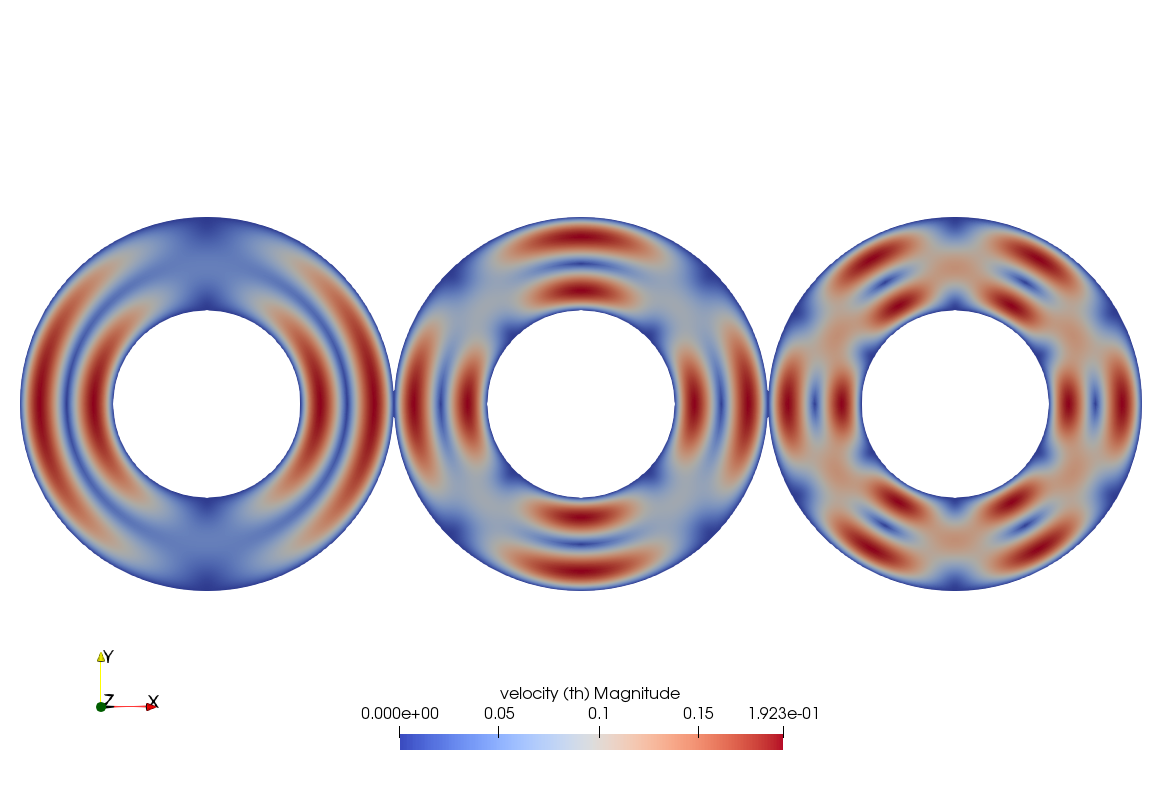
\includegraphics[width=12cm]{python_codes/fieldstone_35/images/vels}\\
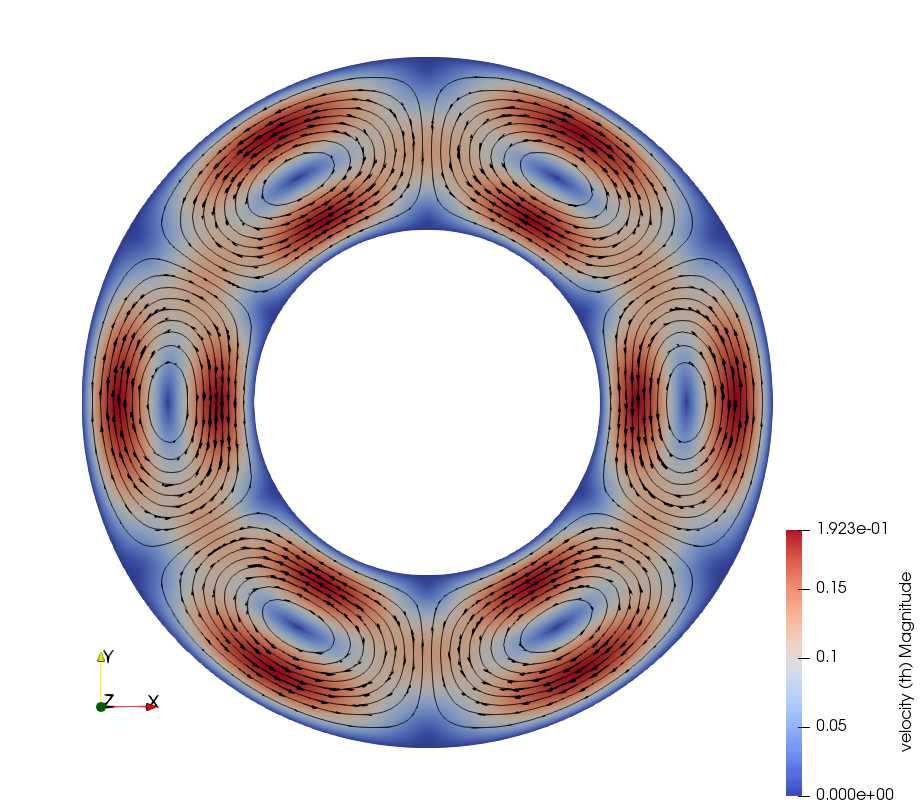
\includegraphics[width=12cm]{python_codes/fieldstone_35/images/psi}\\
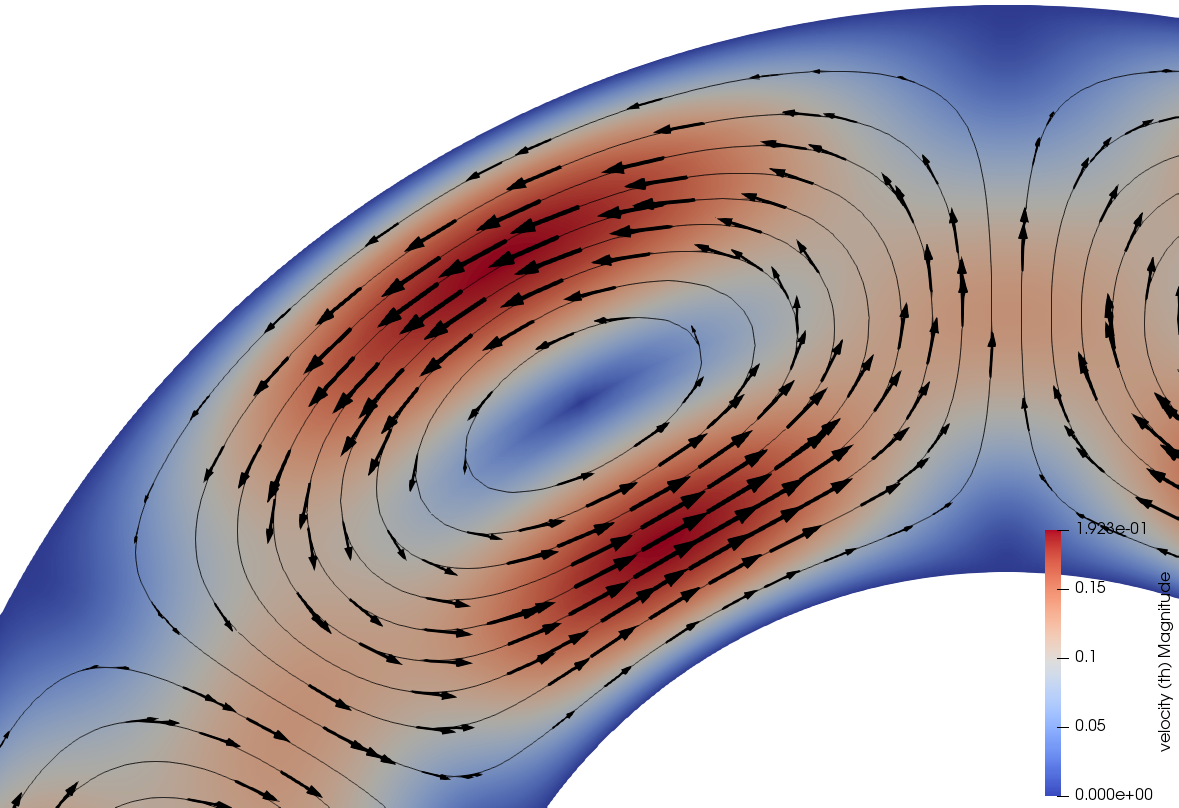
\includegraphics[width=12cm]{python_codes/fieldstone_35/images/psi_arrows}
\end{center}

COMPUTE $f$ from $\phi$ and then the pressure.


%%%%%%%%%%%%%%%%%%%%%%%%%%%%%%%%%%%%%%%%%%%%%%%%%%5
\subsection{Free slip boundary conditions}

Before postulating the form of $\phi(r)$, let us now turn to the boundary conditions that the flow must fulfill, i.e. free-slip on both boundaries.
Two conditions must be met:

\begin{itemize}
\item ${\bm v} \cdot {\bm n}=0$ (no flow through the boundaries) which yields $u(r=R_1)=0$ and $u(r=R_2)=0$, :
\[
\frac{1}{r}\frac{\partial \Psi}{\partial \theta} (r=R_1,R_2)=0   \quad\quad \forall \theta
\]
which gives us the first constraint since $\Psi(r,\theta)=\phi(r)\xi(\theta)$:
\[
\phi(r=R_1)=\phi(r=R_2)=0  
\]
\item $({\bm \sigma} \cdot {\bm n}) \times {\bm n} = {\bm 0} $  (the tangential stress at the boundary is zero)
which imposes: $\sigma_{\theta r}=0$, with
\[
\sigma_{\theta r}=
2 \eta \cdot \frac{1}{2} \left( \frac{\partial v}{\partial r} - \frac{v}{r} + \frac{1}{r} \frac{\partial u}{\partial \theta}    \right)
= \eta \left( \frac{\partial }{\partial r} (- \frac{\partial \Psi}{\partial r}) -
\frac{1}{r} (- \frac{\partial \Psi}{\partial r}) + \frac{1}{r} \frac{\partial }{\partial \theta} (\frac{1}{r}\frac{\partial \Psi}{\partial \theta})    \right)
\]
Finally $\Psi$ must fulfill (on the boundaries!):
\[
-\frac{\partial^2 \Psi}{\partial r^2} + \frac{1}{r}  \frac{\partial \Psi}{\partial r} + \frac{1}{r^2} \frac{\partial^2 \Psi}{\partial \theta^2}=0
\]
\[
- \phi'' \xi + \frac{1}{r} \phi' \xi +  \frac{1}{r^2}  \phi \xi'' = 0
\]
or, 
\[
- \phi''  + \frac{1}{r} \phi'  -k^2  \frac{1}{r^2}  \phi  = 0
\]
Note that this equation is a so-called Euler Differential 
Equation\footnote{http://mathworld.wolfram.com/EulerDifferentialEquation.html}.
Since we are looking for a solution $\phi$ such that $\phi(R_1)=\phi(R_2)=0 $ then 
the 3rd term of the equation above is by definition zero on the boundaries.
We have to ensure the following equality on the boundary:
\[
- \phi''  + \frac{1}{r} \phi'   = 0\quad\quad \text{for} \quad r=R_1,R_2
\]
The solution of this ODE is of the form $\phi(r)=ar^2+b$ and it becomes 
evident that it cannot satisfy $\phi(r=R_1)=\phi(r=R_2)=0$.




\end{itemize}

{\color{red} Separation of variables leads to solutions which cannot fulfill the free slip 
boundary conditions}








